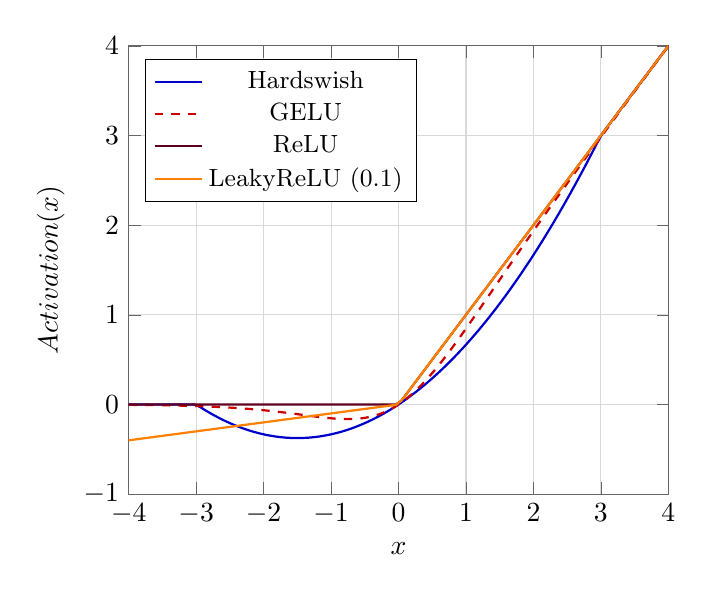
\begin{tikzpicture}
\begin{axis}[
    grid=major,
    xlabel=$x$,
    ylabel=$\text{Activation}(x)$,
    legend pos=north west,
    xmin=-4, xmax=4,
    ymin=-1, ymax=4,
    xtick={-4,-3,...,4},
    ytick={-1,0,...,4},
    legend style={font=\small},
    axis line style={gray!80!black},
    tick style={gray!80!black},
    grid style={gray!30},
]
    % Regular Hardswish
    \addplot[
        thick,
        color=blue!80!black,
        solid,
        samples=100,
        domain=-4:4
    ] {
        max(0,min(6,x+3)) * x / 6
    };
    % GELU Approximation
    \addplot[
        thick,
        color=red!80!black,
        dashed,
        samples=100,
        domain=-4:4
    ] {
        x * (1 / (1 + exp(-1.702 * x)))
    };
    % ReLU
    \addplot[
        thick,
        color=purple!50!black,
        solid,
        samples=100,
        domain=-4:4
    ] {
        max(0,x)
    };
    % LeakyReLU with 0.1 negative slope
    \addplot[
        thick,
        color=orange,
        solid,
        samples=100,
        domain=-4:4
    ] {
        x >= 0 ? x : 0.1*x
    };
    \legend{
        Hardswish,
        GELU,
        ReLU,
        LeakyReLU (0.1)
    }
\end{axis}
\end{tikzpicture}